\chapter{Representação Matricial de Pontos, Vetores e Transformações} %opcional
\label{ape:matrix}
\section{Pontos e Vetores}
Model Matrix

Quando se tratando de pontos no espaço tridimensional que serão transformados de diversas formas, é comum utilizar a notação matricial para pontos e vetores de forma que toda transformação se resume a uma multiplicação de matrizes.

Assim, um ponto $p = (p_x, p_y, p_z)$, é representado por:

\begin{equation}
\begin{bmatrix}
    p_x \\
    p_y \\
    p_z \\
    1 \\
\end{bmatrix}
\end{equation}

Analogamente um vetor $v = (v_x, v_y, v_z)$, é representado por:
\begin{equation}
\begin{bmatrix}
    v_x \\
    v_y \\
    v_z \\
    0 \\
\end{bmatrix}
\end{equation}

O quarto elemento da matriz têm algumas propriedades interessantes, que serão demonstradas adiante, mas um primeiro fato relevante é que a subtração de dois pontos resulta num vetor.

Com essa representação matricial de pontos e vetores surgem tambem representações matriciais para diversos tipos de transformações:


\section{Transformações}
\subsection{Translação}

A matriz que define uma translação de $t_x$ no eixo x, $t_y$ no eixo y e $t_z$ no eixo z é definida da seguinte forma:
\begin{equation}
T = 
\begin{bmatrix}
    1 & 0 & 0 & t_x\\
    0 & 1 & 0 & t_y\\
    0 & 0 & 1 & t_z\\
    0 & 0 & 0 & 1 \\
\end{bmatrix}
\end{equation}

Assim, para aplicar uma transformaçao em um ponto basta multiplicar a matriz pelo ponto:
\begin{equation}
\begin{bmatrix}
    1 & 0 & 0 & t_x\\
    0 & 1 & 0 & t_y\\
    0 & 0 & 1 & t_z\\
    0 & 0 & 0 & 1 \\
\end{bmatrix}
*
\begin{bmatrix}
    p_x \\
    p_y \\
    p_z \\
    1 \\
\end{bmatrix}
=
\begin{bmatrix}
    p_x + t_x\\
    p_y + t_y\\
    p_z + t_z\\
    1 \\
\end{bmatrix}
\end{equation}


Da mesma forma, pode-se aplicar uma matriz de translação a um vetor, tendo o seguinte resultado:
\begin{equation}
\begin{bmatrix}
    1 & 0 & 0 & t_x\\
    0 & 1 & 0 & t_y\\
    0 & 0 & 1 & t_z\\
    0 & 0 & 0 & 1 \\
\end{bmatrix}
*
\begin{bmatrix}
    v_x \\
    v_y \\
    v_z \\
    0 \\
\end{bmatrix}
=
\begin{bmatrix}
    v_x\\
    v_y\\
    v_z\\
    0 \\
\end{bmatrix}
\end{equation}

Percebe-se que pela característica de seu ultimo elemento ser 0, a translação não afeta o vetor, sendo esse o comportamento esperado.

\subsection{Escala}

Outra transformação muito comum é a de escalar vetores e pontos. Escala é uma multiplicação termo a termo dos elementos de uma tripla ordenada por outra. A matrix de escala é definida da seguinte forma:

\begin{equation}
S = 
\begin{bmatrix}
    s_x & 0   & 0   & 0\\
    0   & s_y & 0   & 0\\
    0   & 0   & s_z & 0\\
    0   & 0   & 0   & 1 \\
\end{bmatrix}
\end{equation}

No contexto de pontos, a escala afasta o ponto da origem por um fator $s_x$ no eixo x, $s_y$ no eixo y e $s_z$ no eixo z. A aplicação da matrix no ponto é dada pela equação a seguir:
\begin{equation}
\begin{bmatrix}
    s_x & 0   & 0   & 0\\
    0   & s_y & 0   & 0\\
    0   & 0   & s_z & 0\\
    0   & 0   & 0   & 1 \\
\end{bmatrix}
*
\begin{bmatrix}
    p_x\\
    p_y\\
    p_z\\
    1 \\
\end{bmatrix}
=
\begin{bmatrix}
    p_x * s_x\\
    p_y * s_y\\
    p_z * s_z\\
    1 \\
\end{bmatrix}
\end{equation}


De forma análoga, a matriz de escala muda o tamanho do vetor em cada um de seus eixos, sendo sua aplicação dada pelo valor a seguir.
\begin{equation}
\begin{bmatrix}
    s_x & 0   & 0   & 0\\
    0   & s_y & 0   & 0\\
    0   & 0   & s_z & 0\\
    0   & 0   & 0   & 1 \\
\end{bmatrix}
*
\begin{bmatrix}
    v_x\\
    v_y\\
    v_z\\
    0 \\
\end{bmatrix}
=
\begin{bmatrix}
    v_x * s_x\\
    v_y * s_y\\
    v_z * s_z\\
    0 \\
\end{bmatrix}
\end{equation}


\subsection{Rotação}

Rotações são operações complexas, e portanto uma outra matemática foi desenvolvida para ela, a dos quaterniões, que não será explicada em detalhes no presente relatório. No entanto mesmo que o uso de quaterniões para composição e interpolações seja mais simples, os mesmos são transformados em matrizes de rotação e utilizados da mesma forma que as transformações anteriores. Um exemplo da matriz de rotação mais utilizada que é a rotação de um ângulo $\theta$ por um eixo $u = (u_x, u_y, u_z)$, representada a seguir:

\begin{equation}
R = 
\begin{bmatrix}
    \cos\theta + u_x^2(1-\cos\theta) & u_x u_y (1-\cos\theta) - u_z \sin\theta & u_x u_z (1-\cos\theta) - u_y \sin\theta & 0 \\
     u_y u_x (1-\cos\theta) - u_z \sin\theta   & \cos\theta + u_y^2(1-\cos\theta) & u_y u_z (1-\cos\theta) - u_x \sin\theta    & 0\\
     u_z u_x (1-\cos\theta) - u_y \sin\theta &  u_z u_y (1-\cos\theta) - u_x \sin\theta & \cos\theta + u_z^2(1-\cos\theta)  & 0\\
    0   & 0   & 0   & 1 \\
\end{bmatrix}
\end{equation}

\subsection{Projeção}

Outra transformação muito útil na renderização 3d é a de projeção, sendo a mais utilizada delas a de projeção em perspectiva. A matrix de projeção em perspectiva transforma os pontos de forma que distancias em x e y são afetadas pela posição z. Isso torna-se muito mais claro observando as seguintes imagens:

\begin{figure}[]
  \centering
  \subfloat[Antes]{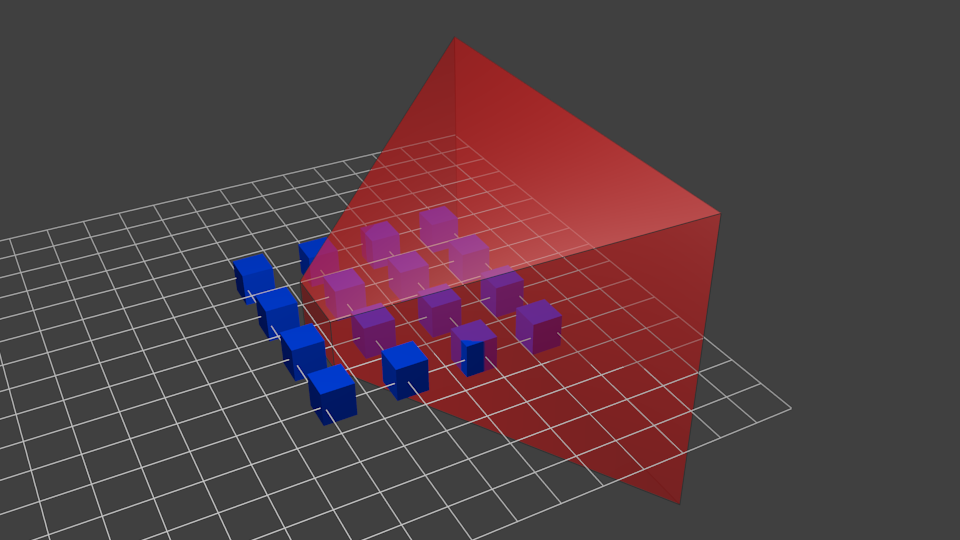
\includegraphics[width=0.45\textwidth]{Ape-Matrizes/perspective-before.png}\label{fig:perspective-before}}
  \hfill
  \subfloat[Depois]{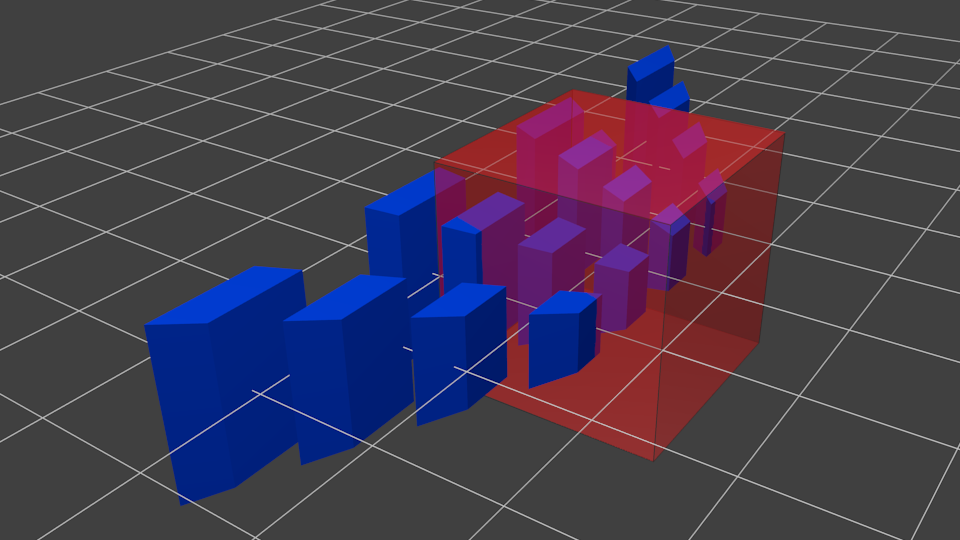
\includegraphics[width=0.45\textwidth]{Ape-Matrizes/perspective-after.png}\label{fig:perspective-after}}
  \caption{Aplicação da matriz de perspectiva a pontos no espaço}
\end{figure}

A matriz de perspectiva geralmente é definida por uma forma conhecida como \textit{frustrum}, um tronco de pirâmide no qual todos os objetos internos são projetados em relação à parte menor. O formato do frustrum pode ser observado na figura \ref{fig:perspective-before}. Para tanto são necessárias alguns parâmetros, a distancia no eixo z do plano proximo (parte menor), representada por $n_z$, a distância no eixo z do plano distante (base), representada por $f_z$, o ângulo de abertura da pirâmide, \textit{fov}, e a razão entre a largura e a altura da base da piramide, representada por \textit{ar}.

Com esses parâmetros, é possível definir a matriz de projeção em perspectiva da seguinte forma:
\begin{equation}
S = 
\begin{bmatrix}
    \frac{1}{ar*\tan(\frac{fov}{2})} & 0 & 0 & 0\\
    0 & \frac{1}{\tan(\frac{fov}{2})} & 0 & 0\\
    0 & 0 & \frac{-n_z-f_z}{n_z-f_z} & 0\\
    0 & 0 & 1 & \frac{2*n_z*f_z}{n_z-f_z}\\
\end{bmatrix}
\end{equation}

